\question{3}{5} Answer the following questions.

\begin{subparts}
  \item Simplify $4(2p-3)-2[p-3(2-q)]+5$.

  \item The diagram shows a trapezium $ABCD$ of height $4$ cm. $AD = x$ cm and $BC = 3x$ cm. Suppose the area of the trapezium is $A$ cm$^2$.
  \par\noindent\hspace*{6em}%
    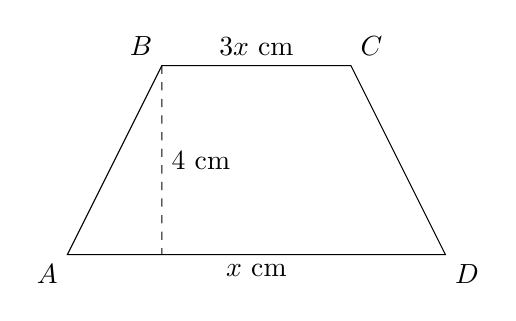
\begin{tikzpicture}[scale=0.8]
      \coordinate (A) at (0,0);
      \coordinate (D) at (6,0);
      \coordinate (B) at (1.5,3);
      \coordinate (C) at (4.5,3);
      \draw (A) -- (B) -- (C) -- (D) -- cycle;
      \draw[dashed] (B) -- (1.5,0);
      \node[below left] at (A) {$A$};
      \node[above left] at (B) {$B$};
      \node[above right] at (C) {$C$};
      \node[below right] at (D) {$D$};
      \node[above] at (3,3) {$3x$ cm};
      \node[below] at (3,0) {$x$ cm};
      \node[right] at (1.5,1.5) {$4$ cm};
    \end{tikzpicture}
  \par
  \begin{subpartsii}
    \item Find a formula for $A$ in terms of $x$.
    \item If $x = 5$, find the area of the trapezium.
  \end{subpartsii}
\end{subparts}

\answerlines{14}
